\begin{figure}[p]
  \centering
  \begin{subfigure}[b]{0.4\linewidth}
    \centering
    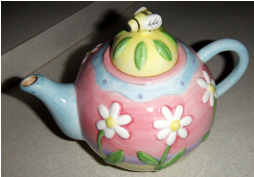
\includegraphics[width=\linewidth]{adversarial-teapot-org}\\
    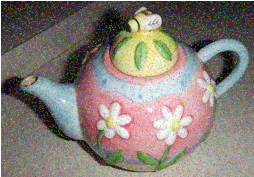
\includegraphics[width=\linewidth]{adversarial-teapot-noisy}
    \caption{Adding 10\% impulse noise to an image of a teapot changes Google Cloud Vision's label from \textit{teapot} (above) to \textit{biology} (below) \citep{Hosseini:2018jr}.}
  \end{subfigure}
  ~
  \begin{subfigure}[b]{0.4\linewidth}
    \centering
    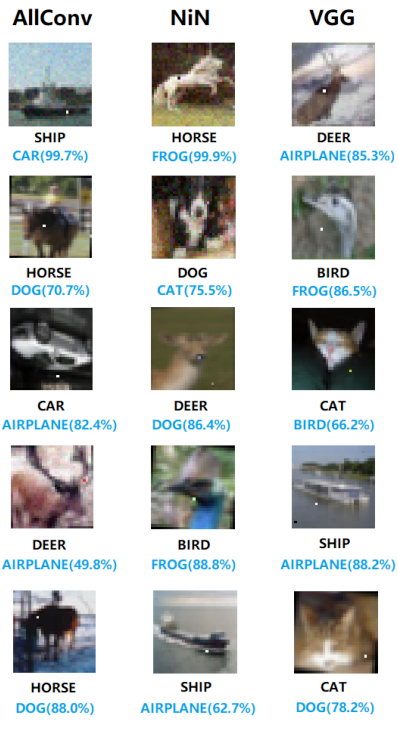
\includegraphics[width=\linewidth]{adversarial-one-pixel}
    \caption{One-pixel attacks applied to three \gls{nn}: AllConv, NiN and VGG \citep{Su:2017uw}.}
  \end{subfigure}
  \\ \bigskip
  \begin{subfigure}[b]{0.8\linewidth}
    \centering
    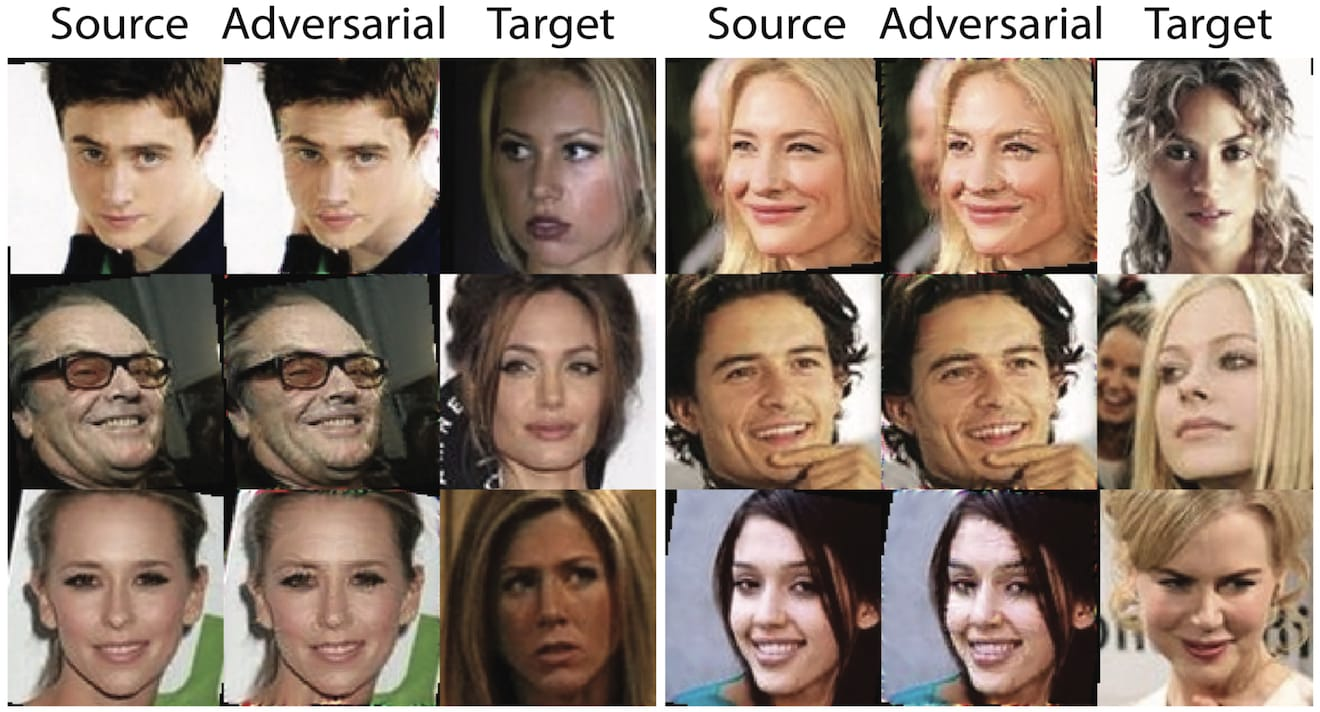
\includegraphics[width=\linewidth]{adversarial-celebrities}
    \caption{Adversarial examples to trick face recognition from the source to target images \citep{Wang:2018vl}.}
  \end{subfigure}

  \caption[Adversarial examples in computer vision]{Sample adversarial examples in state-of-the-art computer vision studies.}
  \label{fig:background:software-quality:reliability-in-cv:adversarial-examples}
\end{figure}